\section{Схемы <<Актёр-критик>>}\label{ActorCriticSection}

\subsection{Бэйзлайн}

При стохастической оптимизации ключевым фактором является дисперсия оценки градиента. Когда мы заменяем мат.ожидания на Монте-Карло оценки, дисперсия увеличивается. Понятно, что замена Q-функции --- выинтегрированных будущих наград --- на её Монте-Карло оценку в REINFORCE \eqref{reinforce_grad} повышало дисперсию. Однако, в текущем виде основной источник дисперсии заключается в другом.

\begin{example}
Допустим, у нас два действия $\A = \{0, 1\}$. Мы породили траекторию, в котором выбрали $a \HM= 0$. Выданное значение <<кредита доверия>> --- пусть это точное значение $Q^{\pi}(s, a \HM= 0)$ --- допустим, равно 100. Это значит, что градиент для данной пары $s, a$ указывает на направление изменение параметров, которые увеличат вероятность $\pi(a \HM= 0 \HM\mid s)$, и это направление войдёт в итоговую оценку градиентов с весом 100. Но 100 --- это много или мало?

Рассмотрим один вес $\theta_i \in \R$ в нашей параметризации стратегии. Без ограничения общности будем считать, что для повышения $\pi(a \HM= 0 \HM\mid s)$ вес $\theta_i$ нужно повышать. Тогда если на следующем шаге оптимизации мы в том же $s$ засэмплировали $a \HM= 1$, то для повышения $\pi(a \HM= 1 \HM\mid s)$ вес $\theta_i$, очевидно, нужно уменьшать (так как сумма $\pi(a \HM= 0 \HM\mid s) \HM+ \pi(a \HM= 1 \HM\mid s)$ обязана равняться 1). С каким весом мы будем уменьшать $\theta_i$? С весом $Q^{\pi}(s, a \HM= 1)$. Что, если оно равно 1000? На прошлом шаге мы шли в одну сторону с весом 100, на текущем --- в другую с весом 1000. За счёт разницы весов мы в среднем движемся в правильную сторону, но нас постоянно дёргает то в одном направлении, то в другом.
\end{example}

\begin{wrapfigure}{r}{0.3\textwidth}
\vspace{-0.5cm}
\centering
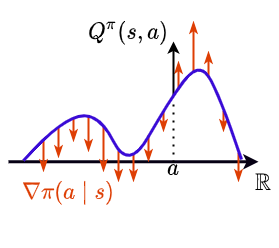
\includegraphics[width=0.3\textwidth]{Images/Baseline.png}
\vspace{-0.9cm}
\end{wrapfigure}

Обобщим описанную в примере ситуацию. Для этого вспомним утверждение \eqref{baseline}: градиент логарифма правдоподобия в среднем равен нулю. Это значит, что если для данного $s$ мы выдаём некоторое распределение $\pi(a \HM\mid s)$, для увеличения вероятностей в одной области $\A$ нужно данный вес $\theta_i$ параметризации увеличивать, а в другой области --- уменьшать. В среднем <<магнитуда изменения>> равна нулю. Но у нас в Монте-Карло оценке только один сэмпл $a \sim \pi(a \HM\mid s)$, и для него направление изменения домножится на кредит, на нашу оценку $Q^{\pi}(s, a)$. Если эта оценка в одной области 100, а в другой 1000 --- дисперсия получаемых значений $\nabla \log \pi(a \HM\mid s) Q^{\pi}(s, a)$ становится колоссальной. Было бы сильно лучше, если бы <<кредит>> --- вес примеров --- был в среднем центрирован, и тоже колебался возле нуля. Тогда для <<плохих действий>> мы правдоподобие этих действий уменьшаем, а для <<хороших действий>> --- увеличиваем, что даже чисто интуитивно логичнее. И для центрирования весов правдоподобия в Policy Gradient методах всегда вводится \emph{бэйзлайн} (baseline), без которого алгоритмы обычно не заведутся.

\begin{proposition}
Для произвольной функции $b(s) \colon \St \to \R$, называемой бэйзлайном, верно:
\begin{equation}\label{pgt_baseline}
\nabla_{\theta} J(\pi) = \frac{1}{1 - \gamma}\E_{d_\pi(s)} \E_{\pi(a \mid s)} \nabla_{\theta} \log \pi_\theta (a \mid s) \left(Q^{\pi}(s, a) - b(s) \right)
\end{equation}
\begin{proof}
Добавленное слагаемое есть ноль в силу формулы \eqref{baseline}. 
\end{proof}
\end{proposition}

Это верно для произвольной функции от состояний и становится неверно, если вдруг бэйзлайн начинает зависеть от $a$. Мы вольны выбрать бэйзлайн произвольно; он не меняет среднего значения оценок градиента, но изменяет дисперсию. 

\begin{theorem}
Бэйзлайном, максимально снижающим дисперсию Монте-Карло оценок формулы градиентов \eqref{pgt_baseline}, является
$$b^*(s) \coloneqq \frac{\E_a \|\nabla_{\theta} \log \pi(a \mid s)\|_2^2 Q^{\pi}(s, a)}{\E_a \|\nabla_{\theta} \log \pi(a \mid s)\|_2^2}$$
\beginproof
Рассмотрим одно состояние $s$ и попробуем вычислить оптимальное значение $b(s)$. Пусть для данного состояния $m$ --- среднее значение оценки градиента, которое, как мы поняли ранее, не зависит от значения $b$:
$$
m \coloneqq \E_{a \sim \pi(a \mid s)} \nabla_{\theta} \log \pi_\theta (a \mid s) Q^{\pi}(s, a)
$$
Для нас будет важно, что $m$ --- просто какой-то фиксированный вектор той же размерности, что и $\theta$. Распишем дисперсию и будем минимизировать её по $b$:
$$\E_a \| \nabla_{\theta} \log \pi(a \mid s) \left( Q^{\pi}(s, a) - b \right) - m \|^2_2 \to \min_{b} $$
Дифференцируем по $b$ и приравниваем к нулю:
$$2 \E_a \left( \nabla_{\theta} \log \pi(a \mid s) \left( Q^{\pi}(s, a) - b \right) - m \right)^T \left(-\nabla_{\theta} \log \pi(a \mid s) \right) = 0 $$
Выделяем норму градиента логарифма правдоподобия:
\begin{equation}\label{optimalbaselineintermediate}
-\E_a \|\nabla_{\theta} \log \pi(a \mid s)\|^2_2 Q^{\pi}(s, a) + \E_a \|\nabla_{\theta} \log \pi(a \mid s)\|^2_2 b + \E_a m^T \left(\nabla_{\theta} \log \pi(a \mid s) \right) = 0
\end{equation}

Осталось заметить, что третье слагаемое есть ноль. Это обобщение нашей теоремы о бэйзлайне: условно, бэйзлайн может быть свой для каждой компоненты вектора $\theta$, опять же, до тех пор, пока он не зависит от действий. В данном случае $m$ --- некоторый фиксированный вектор, одинаковый для всех $a$; поэтому, если $d$ --- размерность вектора параметров $\theta$, то:
$$\E_a m^T \left(\nabla_{\theta} \log \pi(a \mid s) \right) = \E_a \sum_{i=0}^{d} m_i \nabla_{\theta_i} \log \pi(a \mid s) = \sum_{i=0}^{d} m_i \underbrace{\E_a \nabla_{\theta_i} \log \pi(a \mid s)}_{\text{0 по формуле \eqref{baseline}}} = 0$$

Убирая это нулевое третье слагаемое из \eqref{optimalbaselineintermediate}, получаем равенство между первыми двумя:
\begin{equation*}
b\E_a \|\nabla_{\theta} \log \pi(a \mid s)\|^2_2 = \E_a \|\nabla_{\theta} \log \pi(a \mid s)\|^2_2 Q^{\pi}(s, a)
\end{equation*}
Выражая из него $b$, получаем доказываемое.
\end{theorem}

Практическая ценность результата невысока. Знать норму градиента для всех действий $a$ вычислительно будет труднозатратно даже в дискретных пространствах действий. Поэтому мы воспользуемся небольшим предположением: мы предположим, что норма градиента примерно равна для всех действий. Тогда:
$$b^*(s) = \frac{\E_a \|\nabla_{\theta} \log \pi(a \mid s)\|_2^2 Q^{\pi}(s, a)}{\E_a \|\nabla_{\theta} \log \pi(a \mid s)\|_2^2} = \{ \|\nabla_{\theta} \log \pi(a \mid s)\|_2^2 \approx \const(a) \} \approx \E_a Q^{\pi}(s, a) = V^\pi(s)$$

Эта аппроксимация довольно интуитивная: по логике, для дисперсии хорошо, если значения функции $Q^\pi(s, a) \HM- b(s)$ вертятся вокруг нуля, то есть в среднем дают ноль, и поэтому хорошим (но неоптимальным) бэйзлайном будет
$$\E_{a \sim \pi(a \mid s)} \left( Q^{\pi}(s, a) - b(s) \right) \coloneqq 0 \quad \Rightarrow \quad b(s) \coloneqq \E_{a \sim \pi(a \mid s)} Q^{\pi}(s, a) = V^\pi(s)$$

Итак, всюду далее будем в качестве бэйзлайна использовать $b(s) \HM \coloneqq V^\pi(s)$. Подставляя и вспоминая определение \eqref{advantage} Advantage-функции, получаем:
\begin{proposition}
\begin{equation}\label{advantagepg}
\nabla_{\theta} J(\pi) = \frac{1}{1 - \gamma}\E_{d_\pi(s)} \E_{\pi(a \mid s)} \nabla_{\theta} \log \pi_\theta (a \mid s) A^{\pi}(s, a)
\end{equation}
\end{proposition}

Таким образом, <<кредит>>, который мы выдаём каждой паре $s, a$, будет являться оценкой Advantage, и состоять из двух слагаемых: оценки Q-функции и бэйзлайна.

\subsection{Введение критика}

Мы хотели научиться оптимизировать параметры стратегии при помощи формулы градиента, не доигрывая эпизоды до конца. Мы уже поняли, что мат.ожидание по траекториям не представляет для нас проблемы. Тогда осталось лишь придумать, как, не доигрывая эпизоды до конца, проводить credit assignment, то есть определять для каждой пары $s, a$ оценку Advantage-функции.

Раз знание функции $Q^\pi$ позволит обучаться, не доигрывая эпизоды до конца, а функцию в готовом виде нам никто не даст, то возникает логичная идея --- аппроксимировать её. Итак, введём вторую сетку с параметрами $\phi$, которая будет <<оценивать>> наши собственные решения --- \emph{критика} (critic). Сетку, моделирующую стратегию, соответственно будем называть \emph{актёром} (actor), hence the name.

В Policy Gradient алгоритмах в качестве критика обычно учат именно V-функцию. В DQN было обязательным учить именно Q-функцию, так как, во-первых, мы хотели выводить из неё оптимальную стратегию, во-вторых, для уравнения оптимальности Беллмана для оптимальной V-функции фокус с регрессией не прокатил бы --- там мат.ожидание стоит внутри оператора взятия максимума. Сейчас же, в Actor-Critic схеме, мы можем обойтись только V-функцией, поскольку оценить Q-функцию мы можем хотя бы так:
\begin{equation}\label{Qonlineonestep}
Q^\pi(s, a) = r(s, a) + \gamma \E_{s'} V^\pi(s') \approx r(s, a) + \gamma V^\pi(s'), \qquad s' \sim p(s' \mid s, a)
\end{equation}
Иначе говоря, если у нас есть приближение V-функции, то мы можем использовать её как для бэйзлайна, так и для оценки Q-функции. Важно, что V-функция намного проще, чем Q-функция: ей не нужно дифференцировать между действиями.

\begin{example}
Рассмотрим типичную задачу: вы можете перемещаться в пространстве в разные стороны. Если вы отправитесь вправо, через 100 шагов вы получите +1. $Q^*(s, \text{вправо}) \HM= \gamma^{100}$. 

\begin{wrapfigure}{r}{0.3\textwidth}
\vspace{-0.5cm}
\centering
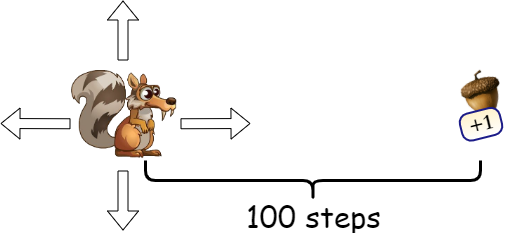
\includegraphics[width=0.3\textwidth]{Images/QisBad.png}
\vspace{-0.9cm}
\end{wrapfigure}

Посмотрим на значение функции в других действиях: например, $Q^*(s, \text{влево}) \HM= \gamma^{102}$. Вот с такой точностью наша $Q^*$ должна обучиться в этом состоянии, чтобы жадная стратегия выбирала правильные действия. Именно поэтому в подобных ситуациях DQN-подобные алгоритмы не срабатывают: из-за проблемы накапливающейся ошибки сигнал на 100 шагов просто не распространяется с такой точностью.
\end{example}

Возможность не обучать сложную $Q^*$ является одним из преимуществ подхода прямой оптимизации $J(\theta)$. Мы из соображений эффективности алгоритма (и задачи снижения дисперсии) не сможем обойтись совсем без обучения каких-либо оценочных функций, но нам хватит лишь $V^{\pi}$, причём ей достаточно лишь понимать, какие области пространства состояний --- хорошие, а какие плохие; нам в целом даже и не требуется, чтобы она это делала с высокой точностью, поскольку главное, чтобы она давала более-менее адекватную оценку совершённых нашим актёром, нашей стратегией, действий.

% Конечно, мы могли бы учить и $Q^{\pi}$ в качестве критика. Для бэйзлайна нам нужно $V^{\pi}(s)$; если у нас есть Q-критик и пространство действий дискретно, то мы можем посчитать $V^\pi$ по формуле \eqref{VQ}. Если пространство действий непрерывно, то возникает затруднение: если бэйзлайн тоже оценивать по Монте-Карло, то от него скорее всего будет не так много толку, и придётся либо вводить третью сетку, учащую $V^\pi(s) \HM= \E_{a \sim \pi(a \mid s)} Q^\pi(s, a)$, либо хотя бы оценивать по Монте-Карло с большим количеством сэмплов, что может быть дороговато. Поскольку без бэйзлайна никуда, это может быть ещё одним аргументом в пользу V-критика. 

\subsection{Bias-variance trade-off}

Обсудим сначала, как критик будет использоваться в формуле градиента по параметрам стратегии \eqref{advantagepg}. Мы собираемся вместо честного advantage подставить некоторую его оценку (advantage estimator):
\begin{equation}\label{advantageestimation}
\nabla_{\theta} J(\pi) \approx \frac{1}{1 - \gamma}\E_{d_\pi(s)} \E_{a \sim \pi(a \mid s)} \nabla_{\theta} \log \pi_\theta (a \mid s) \underbrace{\Psi (s, a)}_{\approx A^{\pi}(s, a)}
\end{equation}

\begin{remark}
Можно ли мы в качестве критика напрямую учить сетку, выдающую аппроксимацию $A^{\pi}(s, a, \phi)$, и использовать её выход в качестве нашей оценки $\Psi (s, a)$? Это не очень удобно хотя бы потому, что в отличие от Q-функций и V-функций, Advantage --- не абстрактная произвольная функция: она должна подчиняться теореме \ref{pr:advantageiszero}. При этом восстановить по advantage-у Q-функцию без знания V-функции нельзя, а значит, для advantage не получится записать аналога уравнения Беллмана, использующего только advantage-функции.
\end{remark}

Мы рассматривали два варианта оценки Q-функции: Монте-Карло и одношаговая оценка через V-функцию \eqref{Qonlineonestep}. И здесь возникает принципиальный момент: любые гарантии на несмещённость градиентов при использовании какой-либо нейросетевой аппроксимации при оценке Q-функции мгновенно теряются, поскольку у нас нет никаких гарантий, что наша оценка Q-функции будет несмещённой, и науке неизвестно, как это можно было бы форсить. При использовании смещённых оценок градиента мы тут же теряем любые гарантии на сходимость стохастической оптимизации к локальному оптимуму или даже вообще хоть куда-нибудь! Единственный способ оценивать Q-функцию несмещённо --- Монте-Карло, но которая требует полных эпизодов и имеет более высокую дисперсию. Соответствующие два <<крайних варианта>> выбора функции $\Psi (s, a)$, соответственно, приобретают такой вид:

\vspace{0.2cm}
\begin{center}
\begin{tabular}{ccc}
\toprule
    \textbf{$\Psi (s, a)$} & \textbf{Дисперсия} & \textbf{Смещение}  \\
\midrule
    $R_t - V^\pi(s)$ & высокая & нету \\
    \hdashline
    $r(s, a) + \gamma V^\pi(s') - V^\pi(s)$ & низкая & большое \\
\bottomrule
\end{tabular}
\end{center}
\vspace{0.2cm}

В таблице идёт речь именно о дисперсии и смещении оценки градиента $J(\pi)$ при использованной аппроксимации! А то есть, в первом случае оценка Q-функции несмещённая, оценка V-функции смещённая, но поскольку в качестве бэйзлайна в силу \eqref{baseline} может использоваться совершенно произвольная функция от состояний, совершенно несущественно, насколько наша аппроксимация $V^\pi(s)$ вообще похожа на истинную оценочную функцию. Во втором же случае, аппроксимация $V^\pi(s')$ используется для оценки Q-функции и вызывает смещение в том числе в оценке градиента. Дисперсия же снижается, поскольку в Q-функции аккумулированы мат.ожидания по всему хвосту траектории; она в обоих случаях существенно ниже, чем до введения бэйзлайна, но замена Монте-Карло оценки на бутстрапированную оценку снижает её ещё сильнее.

На самом деле, есть ещё целое семейство промежуточных вариантов --- \emph{многошаговых} (multi-step) оценок Q-функции. Формально можно сказать, что мы пользуемся N-шаговым уравнением Беллмана \eqref{NstepBellman}, которое для выражения Q-функции через V-функцию с заглядыванием в будущее на следующие N шагов имеет следующий вид:
$$Q^\pi(s_t, a_t) \approx \sum_{t'=0}^{N-1} \gamma^{t'} r_{t + t'} + \gamma^N V^\pi(s_{t + N}) $$
\begin{definition}
\emph{$N$-шаговая оценка Advantage-функции} ($N$-step advantage estimator) определяется как:
\begin{equation}\label{Nstepadvantage}
\Psi_{(N)} (s_t, a_t) \coloneqq \sum_{t'=0}^{N-1} \gamma^{t'} r_{t + t'} + \gamma^N V^\pi(s_{t + N}) - V^\pi(s_t)
\end{equation}
\end{definition}

С ростом $N$ дисперсия такой оценки увеличивается: всё больший фрагмент траектории мы оцениваем по Монте-Карло, нам становятся нужны сэмплы $a_{t+1} \sim \pi(a_{t+1} \mid s_{t=1})$, $s_{t+2} \sim \pi(s_{t+2} \mid s_{t+1}, a_{t+1})$, \dots , $s_{t+N} \sim \pi(s_{t+N} \mid s_{t+N-1}, a_{t+N-1})$. Понятно, что эти сэмплы из буфера получить не получится (действия должны генерироваться из текущей стратегии); а при $N \to \infty$ оценка в пределе переходит в полную Монте-Карло оценку оставшейся награды, где дисперсия большая, но зато исчезает смещение в силу отсутствия смещённой аппроксимации награды за хвост траектории.

Использование многошаговых оценок, которое было невозможно в off-policy режиме --- чуть ли не главное преимущество on-policy режима обучения. Мы можем не дожидаться, пока наш критик идеально обучиться: в оценку Advantage попадает сигнал в том числе из далёкого будущего при больших $N$, и удачно совершённое действие начинает совершаться чаще. Более того мы снижаем смещение наших оценок градиента. Trade-off заключается в том, что чем дальше в будущее мы заглядываем, тем выше дисперсия этих оценок; помимо этого, для заглядывания в будущее на $N$ шагов нужно же иметь это самое будущее, то есть из каждой параллельно запущенной среды понадобится собрать для очередного мини-батча не по одному сэмплу, а собрать целый фрагмент траектории.

\begin{definition}
Фрагмент траектории $s_t, a_t, r_t, s_{t+1}, a_{t+1}, r_{t+1}, \dots, s_{t + N}$ будем называть \emph{роллаутом} (rollout) длины $N$.
\end{definition}

%Без ограничения общности можно в роллаутах индексировать время, начиная с нуля, в силу стационарности. 

Заметим, что мы вовсе не обязаны использовать для всех пар $s, a$ оценку одной и той же длины $N$. То есть мы не должны брать для $s_t, a_t$ из $N$-шагового роллаута $N$-шаговую оценку, а остальные пары $s, a$ из роллаута не использовать в обучении лишь потому, что для них $N$-шаговая оценка невозможна; вместо этого для них следует просто использовать ту многошаговую оценку, которая доступна. Это полностью корректно, поскольку любая $N$-шаговая оценка является оценкой Advantage-а для данного слагаемого в нашей формуле градиента. 

Пока что в нашем алгоритме роллауты не могут быть сильно длинными: пары $s, a$ из длинных роллаутов сильно скоррелированы, что нужно перебивать числом параллельно запущенных сред, и тогда при увеличении длины роллаута начинает раздуваться размер мини-батча. Потом собранные переходы будут использованы всего для одного шага градиентного подъёма, и переиспользовать их будет нельзя; это расточительно и поэтому большой размер мини-батча невыгоден. Поэтому длина роллаутов обычно используется достаточно небольшая, чтобы можно было говорить, что самая выгодная оценка Advantage-а --- оценка максимальной длины: для $s_t$ мы можем построить $N$-шаговую оценку, её и возьмём; для $s_{t+1}$ уже не более чем $N-1$-шаговую; наконец, для $s_{t+N-1}$ нам доступна лишь одношаговая оценка, просто потому что никаких сэмплов после $s_{t+N}$ мы ещё не получали. Пока $N$ не так велико, чтобы дисперсия раздувалась, это самое разумное решение trade-off-а, и о более умном решении пока думать не нужно. 

\begin{definition}
Для пар $s_t, a_t$ из роллаута $s_0, a_0, r_0, s_1, a_1, r_1, \dots, s_N$ длины $N$ будем называть \emph{оценкой максимальной длины} (max trace estimation) оценку с максимальным заглядыванием в будущее: для Q-функции
\begin{equation}\label{maxtrace}
y^{\mathrm{MaxTrace}} (s_t, a_t) \coloneqq \sum_{t'=t}^{N-1} \gamma^{t'-t} r_{t'} + \gamma^{N-t} V^\pi(s_N),
\end{equation}
для Advantage функции, соответственно:
\begin{equation*}%\label{maxtraceadvantage}
\Psi^{\mathrm{MaxTrace}} (s_t, a_t) \coloneqq y^{\mathrm{MaxTrace}} (s_t, a_t) - V^\pi(s_t)
\end{equation*}
\end{definition}

\subsection{Обучение критика}

Как обучать критика $V^\pi$? Воспользуемся идеей перехода к регрессии, которую мы обсуждали раньше в контексте DQN (раздел \ref{toregression}). Нам нужно просто решать уравнение Беллмана \eqref{VV}:
$$V^\pi(s, \phi_{k+1}) \leftarrow \E_{a} \left[ r(s, a) + \gamma \E_{s'} V^\pi(s', \phi_k) \right]$$

Однако, давайте воспользуемся преимуществами on-policy режима и поймём, что мы можем поступить точно также, как с оценкой Q-функции в формуле градиента, и решать многошаговое уравнение Беллмана вместо одношагового. Возможность таким образом бороться с проблемой \emph{накапливающейся ошибки} (compound error) чуть ли не главное преимущество policy gradient подхода: если раньше для распространения награды, полученной в некоторый момент времени, на 100 шагов в прошлое, понадобилось бы провести 100 этапов метода простой итерации, когда каждый этап задача регрессии решается в сильно неидеальных условиях, и ошибка аппроксимации накапливается, то теперь, используя двухшаговые оценки, методу простой итерации понадобится уже 50 этапов, а если десятишаговые --- то всего 10. А если мы Монте-Карло оценки используем, то вообще нет такой проблемы! Другая появляется с ростом $N$ --- таргет в задаче регрессии становится всё более и более шумным. Конечно же, это в точности тот же самый trade-off, что и при оценке Q-функции в формуле градиента.

Мы можем для оценки Q-функции для обучения политики и для построения целевой переменной для критика использовать разные подходы (оценки разной длины), но особого смысла в этом немного: хороший вариант для одного будет хорошим вариантом и для другого. Поэтому можно считать, что если мы оцениваем Advantage как
$$\Psi(s, a) = y - V_{\phi}^{\pi}(s),$$
где $y$ --- некоторая оценка Q-функции, то $y$ же является и таргетом для V-функции. Используя функцию потерь MSE с таким таргетом, мы как раз и учим среднее значение наши оценок Q-функции, то есть бэйзлайн.

% Однако, если мы учим Q-функцию, мы в формуле градиента \eqref{gradient} сможем в случае дискретных пространств состояний взять мат.ожидание по действиям
% $$\E_{a \sim \pi(a \mid s)} \nabla_{\theta} \log \pi_\theta (a \mid s) Q^{\pi}(s, a)$$
% а если мы учим только V-функцию, то сможем применить оценку \eqref{Qonlineonestep} только для одного действия из траектории; то есть, оценивать $\E_{a \sim \pi(a \mid s)}$ придётся по Монте-Карло, а это немного повысит дисперсию.

% Итак, для каждого варианта напишем, что у нас является входом, что искомой функцией (это всегда правая часть соответствующего уравнения Беллмана, которое мы хотим решить методом простой итерации), что целевой переменной (она должна быть вычислима и являться несмещённой оценкой какого-либо мат.ожидания, стоящего в искомой функции) и от каких случайных величин она зависит (это ключевой фактор, так как от этого зависит, сможем ли мы, например, использовать реплей буфер). Функция потерь во всех случаях должна учить мат.ожидания, поэтому MSE.

% \vspace{0.2cm}
% \begin{center}
% \begin{tabular}{ccccc}
% \toprule
%     \textbf{Что учим?} & \textbf{Вход} & \textbf{Искомая функция} & \textbf{Требуемые сэмплы} & \textbf{Целевая переменная}  \\
% \midrule
%     $V^{\pi}(s)$ & $s$ & $\E_{a} \left[ r + \gamma \E_{s'} V^\pi(s', \omega_k) \right]$ & \begin{tabular}{@{}c@{}}$a \sim \pi(a \mid s)$ \\ $s' \sim p(s' \mid s, a)$\end{tabular} & $r + \gamma V^\pi(s', \omega_k)$ \\
%     \hdashline
%     $Q^{\pi}(s, a)$ & $s, a$ & $ r + \gamma \E_{s'} \E_{a'} Q^\pi(s', a', \omega_k)$ & \begin{tabular}{@{}c@{}}$s' \sim p(s' \mid s, a)$ \\ $a' \sim \pi(a' \mid s')$\end{tabular} & $r + \gamma Q^\pi(s', a', \omega_k)$ \\
%     \hdashline
%     $Q^{\pi}(s, a)$ & $s, a$ & $ r + \gamma \E_{s'} \E_{a'} Q^\pi(s', a', \omega_k)$ & $s' \sim p(s' \mid s, a)$ & $r + \gamma \E_{a'} Q^\pi(s', a', \omega_k)$ \\
% \bottomrule
% \end{tabular}
% \end{center}
% \vspace{0.2cm}

% В последнем случае пространство действий должно быть дискретно, чтобы в целевой переменной взялось $\E_{a'}$, то есть выбор между вторым и третьим вариантом определяется только этим.

% Подумаем, каких критиков мы можем обучать с буфера. При обучении $V^\pi$ нам опять нужна для данного $s$ пара $a \sim \pi, s' \sim p(s' \mid s, a)$, поэтому $V$-критика также не удастся обучать по буферу. При обучении $Q^\pi$ нам нужно для взятых из буфера $s, a$ иметь сэмпл $s'$ (пожалуйста --- в силу однородности среды) и $a'$ из текущей политики, который всегда можно сгенерировать онлайн (или мат.ожидаем по $a'$ из текущей политики, если есть такая возможность). Значит, $Q$-критика можно обучать с буфера.

Брать для обучения критика набор выходных состояний $s$ мы можем откуда угодно. Поэтому для удобства будем брать $s \HM\sim \mu_\pi(s)$, чтобы можно было использовать для обучения критика и актёра один и тот же мини-батч. Итого получаем следующее: делаем несколько шагов взаимодействия со средой, собирая таким образом роллаут некоторой длины $N$; считаем для каждой пары $s, a$ некоторую оценку Q-функции $y(s, a)$, например, оценку максимальной длины \eqref{maxtrace}; оцениваем Advantage каждой пары как $\Psi(s, a) \HM \coloneqq y(s, a) - V^{\pi}_{\phi}(s)$; далее по Монте-Карло оцениваем градиент по параметрам стратегии
$$\nabla_\theta J(\pi) \approx \frac{1}{N} \sum_{s, a} \nabla_{\theta} \log \pi_\theta (a \mid s) \Psi(s, a)$$
и градиент для оптимизации критика (допустим, критик --- Q-функция):
$$\Loss^{\critic}(\phi) = \frac{1}{N} \sum_{s, a} \left( y(s, a) - V^{\pi}_{\phi}(s) \right)^2$$
Естественно, для декорреляции нужно собрать несколько независимых роллаутов из параллельно запущенных сред.

\begin{remark}
Когда состояния представлены в виде картинок, понятно, что и критику, и актёру нужны примерно одни и те же фичи с изображений (положение одних и тех же распознанных объектов). Поэтому кажется, что если критик и актёр будут двумя разными сетками, их первые слои будут обучаться одному и тому же. Логично для ускорения обучения объединить \emph{экстрактор фич} (feature extractor) для критика и актёра и сделать им просто свои индивидуальные головы. Конечно, тогда нужно обучать всю сеть синхронно, но мы специально для этого считаем градиенты для актёра и критика по одному и тому же мини-батчу. Есть у такого \emph{общего позвоночника} (shared backbone) и свои минусы: лоссы придётся отмасштабировать при помощи скалярного гиперпараметра $\alpha$ так, чтобы одна из голов не забивала градиентами другую:
$$\Loss^{\mathrm{ActorCritic}}(\theta) = \Loss^{\actor}(\theta) + \alpha \Loss^{\critic}(\theta)$$
\end{remark}

\subsection{Advantage Actor-Critic (A2C)}

Мы собрали стандартную схему Advantage Actor Critic (A2C): алгоритма, который работает в чистом виде on-policy режиме.

\begin{algorithm}{Advantage Actor-Critic (A2C)}
\textbf{Гиперпараметры:} $M$ --- количество параллельных сред, $N$ --- длина роллаутов, $V^\pi$ --- нейросеть с параметрами $\phi$, $\pi$ --- нейросеть для стратегии с параметрами $\theta$, $\alpha$ --- коэф. масштабирования лосса критика, SGD оптимизатор.

\vspace{0.3cm}
Инициализировать $\theta, \phi$ \\
\textbf{На каждом шаге:}
\begin{enumerate}
    \item в каждой параллельной среде собрать роллаут длины $N$, используя стратегию $\pi_{\theta}$:
    $$s_0, a_0, r_0, s_1, \dots , s_N$$
    \item для каждой пары $s_t, a_t$ из каждого роллаута посчитать оценку Q-функции максимальной длины, игнорируя зависимость оценки от $\phi$:
    $$Q^\pi(s_t, a_t) \coloneqq \sum_{t' = t}^{N-1} \gamma^{t' - t} r_{t'} + \gamma^{N - t} V^\pi_{\phi}(s_N)$$
    \item вычислить лосс критика:
    $$\Loss^{\critic}(\phi) \coloneqq \frac{1}{MN}\sum_{s_t, a_t} \left( Q^\pi(s_t, a_t) - V^\pi_\phi(s_t) \right) ^2$$
    \item вычислить градиент для актёра:
    $$\nabla^{\actor}_\theta \coloneqq \frac{1}{MN}\sum_{s_t, a_t} \nabla_\theta \log \pi_\theta(a_t \mid s_t) \left( Q^\pi(s_t, a_t) - V^\pi_\phi(s_t) \right) $$
    \item сделать шаг градиентного спуска по градиенту $-\nabla^{\actor}_\theta + \alpha \nabla_\phi \Loss^{\critic}(\phi)$
\end{enumerate}
\end{algorithm}

\begin{example}
Перерыв на \href{https://hackernoon.com/intuitive-rl-intro-to-advantage-actor-critic-a2c-4ff545978752}{чтение комиксов}.
\end{example}

